\section{GUI plotting performance}
    We evaluated the performance of the GUI plotting routine for an observed $\Delta$Q. The routine first prepares the $\Delta$Q, creating vectors QPointF (a Qt class representing a point for a QtChart), representing the x and y values of the $\Delta$Qs CDF. The vectors are created for the lower bound, the upper bound the mean of the window of $\Delta$Qs and the observed $\Delta$Q.

    Then, once the vectors are prepared, Qt replaces the old points with the new points for every element being plotted.

    \begin{figure}[H]
        \begin{center}
            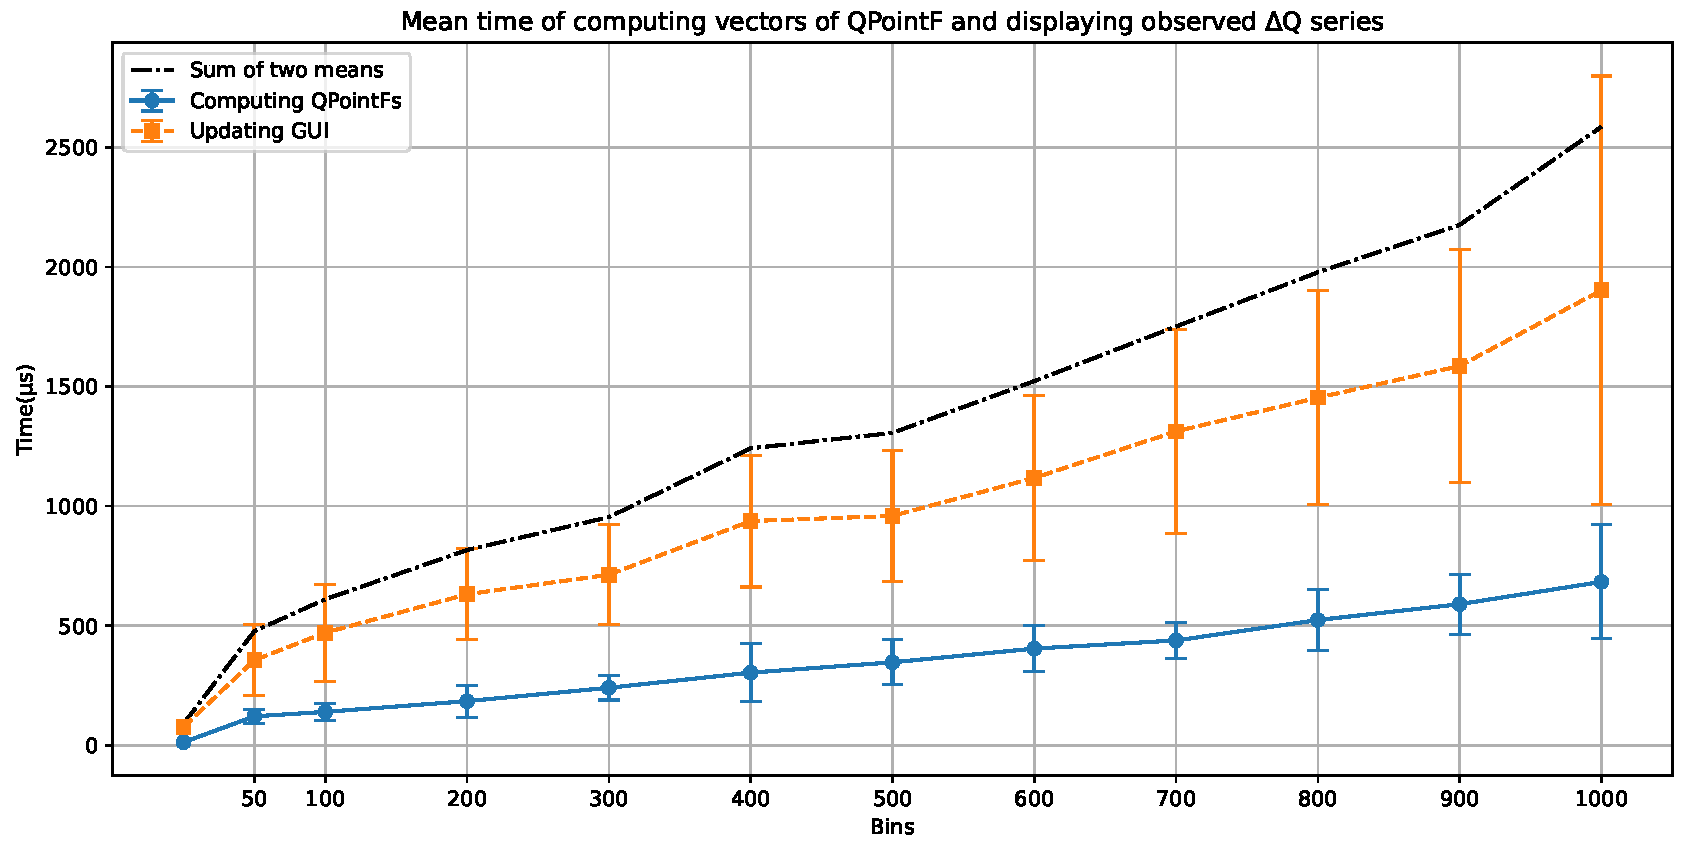
\includegraphics[width = 0.85\textwidth]{img/plots.pdf}
        \end{center}
    \end{figure}

    The result scales up to 2 ms for 1000 bins, since multiple plots have to be shown, if the probe observes the causal relationships of outcome and operators, the calculated $\Delta$Q will need to be plotted too, the time increase will be twofold. 
    If a user decides to have finer grained representations and multiple plots at once, decreasing (decreasing or increasing?) the polling rate will avoid the plots frame skipping.
